\documentclass[a4paper, dvipsnames, table]{article} 
%pensavo di usare table per i nomi in copertina
\usepackage[utf8]{inputenc}
\usepackage[T1]{fontenc}
\usepackage[italian]{babel}
\usepackage{graphicx}
\usepackage{fancyhdr}

\pagestyle{fancy}

\begin{document}
\title{Burgheria Padovana}
\date{Anno accademico: 2020/2021}

\newpage  %includere repo github?
\begin{figure}
	\centering
	
\includegraphics[width=2cm]{../img/burger-icon.png}%da sistemare qualità
\end{figure}
\maketitle

\begin{table}
	\centering
	\begin{tabular}{c|c c c}
		\textbf{Componenti}
			& Albiero	& Davide      & 1193425 \\
			& Fincato	& Alessandro  & 1201264 \\
 			& Panighel	& Cristiano   & 1201284 \\
			& Tossuto	& Matteo      & 1193493 \\
	\end{tabular}
\end{table}

\begin{center}
	\textbf{Indirizzo sito web}: \\
	\textbf{Email referente del gruppo}: davide.albiero@studenti.unipd.it
\end{center}

\begin{table}
	\centering
	\begin{tabular}{c|c c}
		\textbf{Utenti} & \textbf{Nickname} & \textbf{Password} \\
		\hline
		Admin           & admin & admin             \\
		User            & user  & user              \\
	\end{tabular}
\end{table}

\newpage
	\tableofcontents

\newpage
\section{Introduzione}
	Il progetto \emph{Burgheria Padovana} vuole implementare un sito Internet che offra la possibilità di fornire informazioni riguardo il suo punto vendita.\\
Il locale è aperto già da diversi anni e ha finalmente deciso di rinnovarsi creando un proprio sito internet.\\
Il sito dovrà contenere informazioni riguardanti i panini che offre, suddivisi nelle varie categorie: Pollo, Manzo e Speciali. 
Inoltre conterrà gli eventi a cui sarà possibile partecipare, la storia del locale, gli orari di apertura e come contattare il locale.\\
Il sito permette ad un utente privilegiato (admin) di inserire o eliminare gli eventi e di controllare ed eliminare i commenti degli altri utenti. Gli utenti normali (user) saranno visitatori 
con privilegi minimi per poter inserire od eliminare i propri commenti oltre a poter visitare il sito normalmente.\\
Gli \emph{user} dovranno effettuare la registrazione o il login prima di poter usufruire dei privilegi.\\
Inoltre deve essere garantita l'accessibilità in modo che chiunque possa navigare nel sito senza problemi e tranquillamente.\\
Terminato con l'accessibilità, si pone l'attenzione sull'usabilità: rispettando la separazione tra struttura, presentazione e comportamento e rispettando gli standard \emph{W3C} per quanto riguarda \emph{HTML} e \emph{CSS}.\\
Il sito dovrà garantire una navigazione fluida agli utenti evitando disorientamento e, nel caso accadesse, fornirgli supporto per tornare al sito.\\
	
\newpage
\section{Analisi}
	\subsection{Studio dell'utenza finale}
		Il locale Burgheria Padovana offre un prodotto internazionale, comodo, veloce e buono.\\
Pertanto il sito è pensato per rivolgersi ad una categoria di utenti eterogenei, ad esempio: da consumatori abituali a chi vuole provare qualcosa di nuovo, da chi ha bisogno di mangiare qualcosa al volo a chi vuole gustarsi un buon pasto con calma.\\
Queste categorie di utenti, con privilegi minimi, verrà denominata come \emph{utente generico}.
Mentre l'utente con privilegi verrà denominato come \emph{amministratore}.\\ 
Entrambe le tipologie potranno accedere ai loro privilegi autenticandosi tramite form di login.\\
Essendo un utenza finale generica, sarà necessario utilizzare un linguaggio informale, semplice e comprensibile.
Allo stesso modo si andrà a creare un sito di struttura e layout semplici e simili ai modelli a cui l'\emph{utente generico} è abituato.
Si cercherà, quindi, di non rompere le convenzioni esterne e offrendo, indipendentemente dal browser o dal dispositivo utilizzato, una navigazione veloce e intuitiva.\\
	\subsection{Casi d'uso}
		\subsubsection{Utente generico}
			%cosa può fare l'utente
		\subsubsection{Amministratore}
			%cosa può fare di diverso dagli utenti generici

\newpage
\section{Progettazione}%Obiettivi? Design e DB
	\subsection{Obiettivi}
	\subsection{Design}%layout per differenza tra desktop e mobile?
	\subsection{Database}
		Una parte fondamentale del progetto è il database, in quanto è usato per contenere le informazioni che veranno poi usate dal sito.\\
È stato pensato di creare un database con la funzione di contenere tutti i dati relativi ai prodotti in vendita compresi i voti e i commenti, agli eventi a cui è possibile partecipare e i dati degli utenti registrati.\\
Come si può vedere dalla \emph{Figura \ref{Fig:schemadb}}, le tabelle sono sei:
\begin{itemize}
		\item \textbf{Eventi:} contiene il titolo, la data, il luogo e la descrizione degli eventi a cui sarà possibile partecipare
		\item \textbf{Categoria:} contiene il nome delle categorie
		\item \textbf{Prodotti:} contiene il nome, l'immagine, gli ingredienti e la descrizione dei prodotti venduti
		\item \textbf{Utenti:} contiene l'username e la password degli utenti iscritti. Inoltre si verifica se l'utente è un admin.
        \item \textbf{Voti:} contiene i voti degli utenti
        \item \textbf{Commenti:} contiene i commenti degli utenti
\end{itemize}
\begin{figure}[!h]
	\centering	% L'immagine aggiornata è presente nel branch Main
	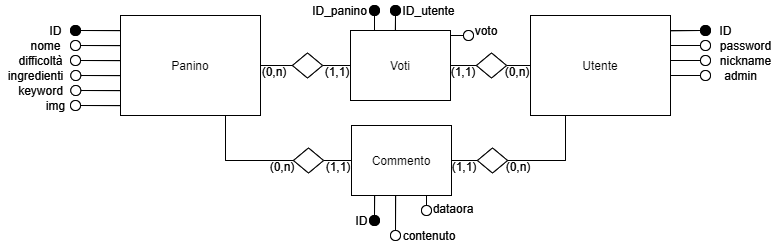
\includegraphics[width=0.7\linewidth]{../database/DiagrammaER.png}\\
    \caption{Schema concettuale database}
	\label{Fig:schemadb}
\end{figure}
Il database viene interrogato da PHP quando bisogna utilizzare o richiamare le informazioni.
Le pagine: \emph{Eventi}, \emph{I nostri Burger}, \emph{Panino} sono riempite dinamicamente tramite chiamata \emph{PHP}.\\
Come spiegato nella sezione \emph{Analisi}, esistono due tipi di utenti: \emph{utente generico} e \emph{amministratore}. Nel database viene utilizzato un booleano per differenziare le due tipologie.\\ 

\newpage
\section{Presentazione}%Per spiegare scelte generali o particolari nel CSS
	\subsection{Desktop}
	\subsection{Mobile}
	\subsection{Stampa}

\newpage
\section{Implementazione}%Per spiegare scelte per HTML, PHP e JS
	\subsection{Linguaggi}
		\subsection{HTML5 e CSS}
		\subsection{MySQL}
			\subsection{MySQL}
Per il mantenimento e salvataggio dei dati e delle informazioni, si è deciso di utilizzare \emph{MySQL}\\
Per le funzioni che necessitano l'uso di \emph{MySQL} viene implementato l'estensione \emph{mysqli}\\
Il database utilizzato è descritto nel capitolo 3: \emph{Progettazione -> Database}.
\\
Da notare che alcuni campi per l'inserimento hanno una grandezza maggiore di quella limite imposta all'utente. 
Questo per assicurarci che anche usando tag HTML, dato che in \emph{MySQL} i simboli "<" e ">", le lettere accentate e caratteri speciali vengono tradotti occupando più spazio, ci sia il rischio che l'input non venisse accettato dal DB portando ad un rifiuto dell'inserimento.
		\subsection{PHP}
		\subsection{JavaScript}

\newpage
\section{Validazione}%Strumenti per la validazione
	\section{Validazione}
La validazione è uno passo fondamentale del progetto, poiché serve a verificare che siano rispettati gli standard \emph{W3C} per quanto riguarda \emph{HTML} e \emph{CSS}.\\
Infatti rispettarli assicura un codice pulito, corretto e che favorisca l'accessibilità e l'usabilità.\\
Inoltre assicura:
\begin{itemize}
	\item Un alto livello di compatibilità tra i diversi browser, rendendo minime o nulle le differenze di visualizzazione del sito, sempre considerando la possibile versione del browser utilizzato dall'utenza a cui ci si riferisce;
	\item Essendo valido non dovrebbe contenere errori e quindi la navigazione risulta più veloce e fluida;
	\item Un sito valido e senza errori non viene interpretato dal browser "a modo suo" ma rispetta "il volere" degli sviluppatori comportandosi come previsto da questi ultimi;
	\item Un sito valido e senza errori viene indicizzato in modo positivo dal browser;
	\item Un sito più accessibile e usabile.
\end{itemize}
Per validare il sito sono stati utilizzati i seguenti strumenti:
\begin{itemize}
	\item \textbf{W3C HTML Validator}\\
	Indirizzo sito web: \url{https://validator.w3.org/}\\
	È un servizio gratuito di \emph{W3C} che consente di validare le pagine \emph{HTML}.
	La validazione può avvenire in tre modi: attraverso il caricamento del file da validare, facendo copia e incolla del codice da validare o inserendo l'indirizzo della pagina se quest'ultima si trova online.\\
	Se il codice non è valido, viene segnalato il numero di errori, il loro tipo e a quale riga e colonna della pagina sono stati trovati.
	\item \textbf{W3C CSS Validator}\\
	Indirizzo sito web: \url{https://jigsaw.w3.org/css-validator/}\\
	È un servizio gratuito di \emph{W3C} che consente di validare il \emph{CSS}.\\
	Anche in questo caso i metodi di validazione sono tre come nel sito precedente.\\
	La segnalazione degli errori viene gestita nell'identico modo del sito precedente.\\
	 \item In entrambi i siti, se le pagine e il codice risultano validi, riportano del codice \emph{HTML} per poter utilizzare delle immagini, del \emph{W3C},che certificano la validazione del sito.
\end{itemize}

\newpage
\section{Fase di Test e Strumenti}%Dove e con cosa testato
	\subsection{XAMPP}
		\subsection{XAMPP}
\emph{XAMPP} è una distribuzione di Apache che permette, tra le varie funzioni, l'utilizzo di \emph{MySQL} e \emph{PHP} di cui abbiamo usufruito.\\
Il loro utilizzo ci ha permesso di realizzare in locale la parte dinamica del sito e la parte di Database, testando le richieste \emph{PHP} e le interrogazioni \emph{MySQL}.
	\subsection*{Silktide - Toolbar}	
	
\newpage
\section{Suddivisione del lavoro}

\end{document}